\subsection{TPC reconstruction, calibration, and data compression}
\label{sec:calibreco:reco:overview}

The ALICE upgrade requires a major change of the computing concept in
order to be able to process and store the large amount of data
produced in \pbpb collisions. The main contributor to the data volume
will be the TPC operated in continuous readout mode.
Most of the data processing and reconstruction will be performed on the
computing cluster of the new online systems~\cite{ALICELOI}.
New requirements to calibration and reconstruction algorithms emerge in
terms of running stability, processing time, memory consumption, as well
as parallelizability on different levels.
A massive use of hardware co-processors, such as FPGAs for the early
processing steps, as well GPGPUs\footnote{General-Purpose Graphics
Processing Units (GPGPUs)} for the later processing is foreseen.
These requirements build strict constraints on the data reconstruction
and calibration, as well as data compression.


%===================================================================
% \subsubsection{The TPC in the general reconstruction scheme}
\subsubsection{Overview of the TPC reconstruction scheme}
\label{sec:calibreco:intro:reco}


The choice of the reconstruction algorithms is strongly driven
by the constrains of the online processing.
However, in the discussion below we will focus on demonstrating the
overall strategy and the general feasibility of online reconstruction
under the operational conditions expected in \run{3}.

A two-stage process, as depicted in
\figref{fig:calibreco:calib:intro:flow}, is foreseen for the online data
processing.
The first stage (see \cite{TPCTDR}) will focus on
cluster finding and the association of clusters to tracks, which are
needed in order to perform the necessary data size reduction.
% This stage must be performed online.
The compressed data will be written to permanent storage.
The reconstructed tracks have sufficient precision to allow the matching
to the external detectors, mainly ITS and TRD, to improve the quality of
the calibration during the next reconstruction stage.

\begin{figure}[htp]
  \begin{center}
    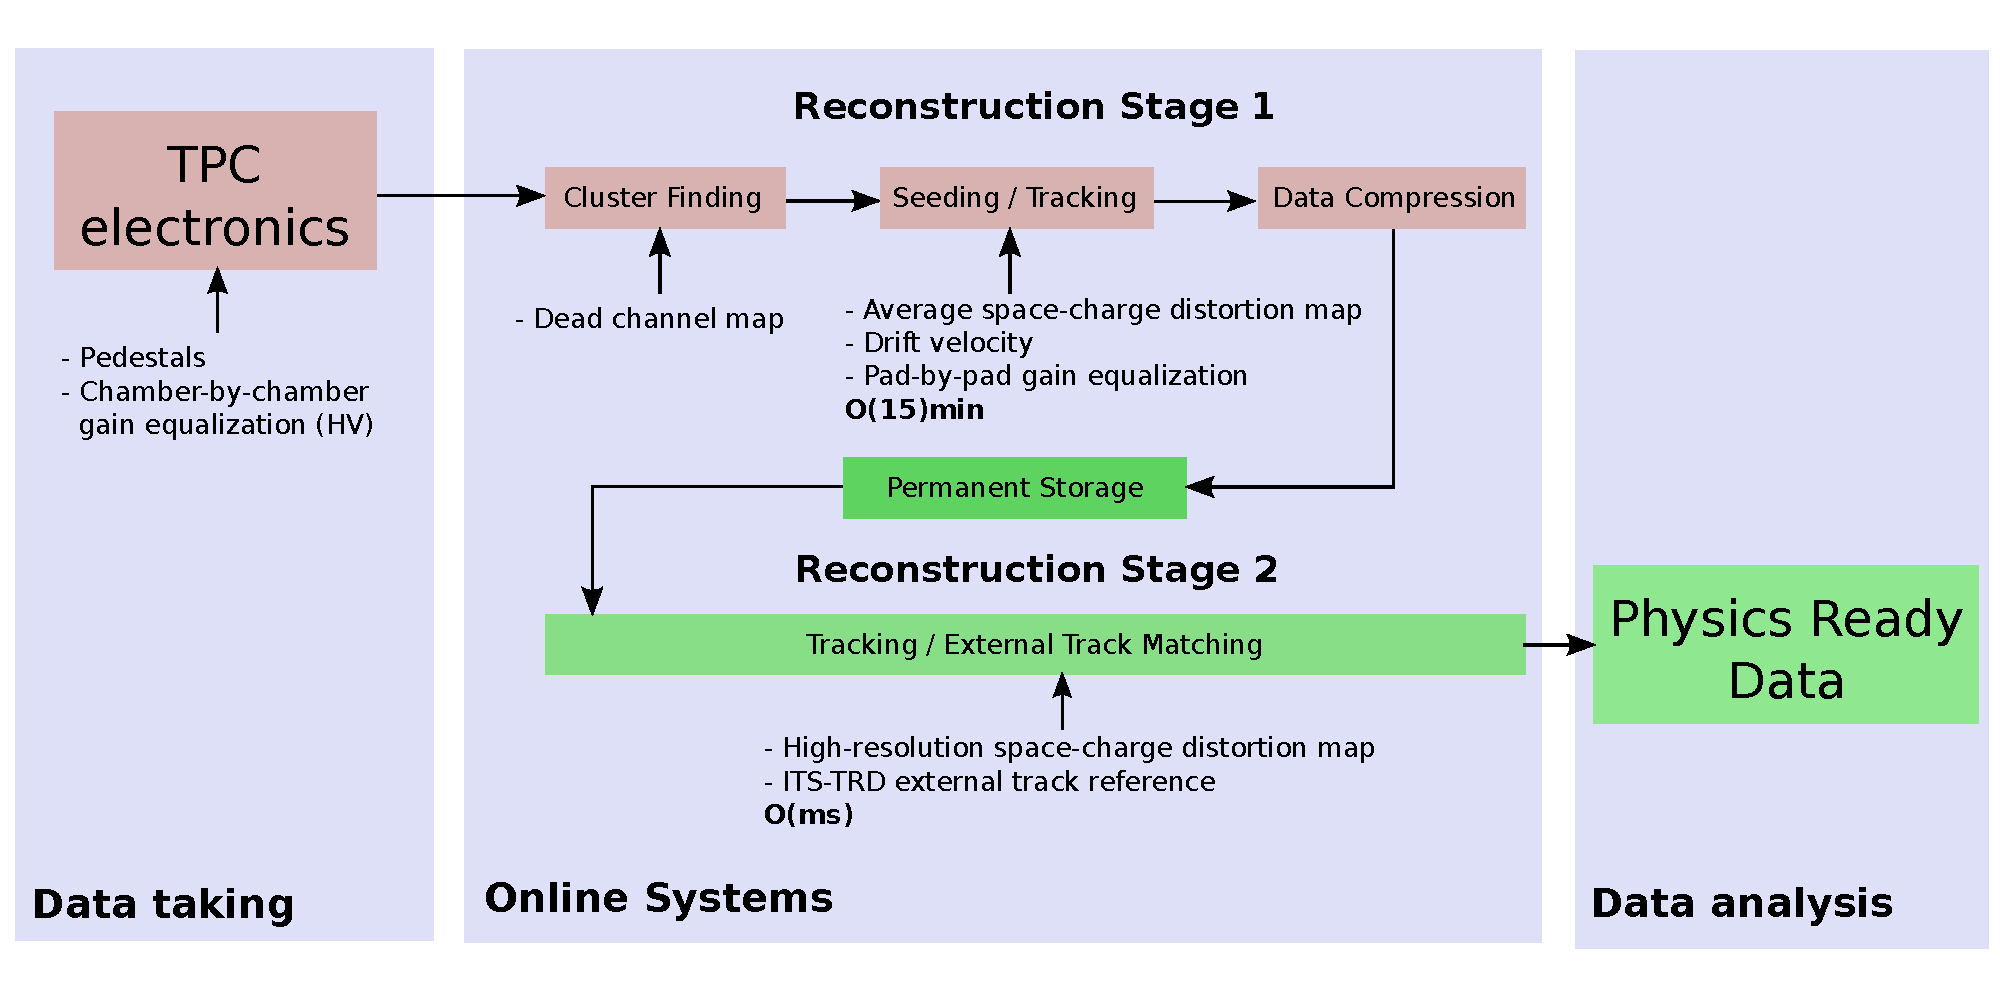
\includegraphics[width=0.9\textwidth]{TPC/CalibSteps}
    \caption[Schematic outline of the calibration flow]{Schematic
      outline of the calibration flow during the data-taking and
      reconstruction process.}
    \label{fig:calibreco:calib:intro:flow}
  \end{center}
\end{figure}

The second reconstruction stage will also be performed on the online
computing cluster, but in an asynchronous mode and can thus be repeated
at any time.
It aims at a further improvement of the data quality, in particular in
terms of the space-charge distortion calibrations, and employs
information from external detectors as well as more detailed calibration
data.

\subsubsection{Data size and data compression}
\label{sec:calibreco:intro:compression}

After zero suppression on the level of the \fee, the average TPC raw
data size in \minbias \pbpb interactions is $\sim20\,$MB.
At an interaction rate of
50\,kHz, this would result in an input rate of about
1\,TB/s to the online systems, and a total amount
of
3\,EB ($10^{18}$\,Byte) of TPC data in \run{3}. Such numbers
exceed the predicted available bandwidth and storage space by a large
factor. Thus, in order to permit permanent data storage, additional
compression on top of zero suppression to below 1\,MB per
interaction is required. This can be achieved by two levels of pattern
recognition that are performed in the online systems.

The zero-suppressed raw data are decoded at the input to the online
farm, where the raw data digits (arrival time at the \fee and signal
amplitude) are associated with the corresponding geometrical position
(pad row and pad coordinates). Cluster finding is performed
on the digits, which produces three-dimensional charge clusters.
This first step is carried out on the FLPs.

As the radial coordinate is fixed by the well-separated pad
rows, cluster finding is reduced to a two-dimensional problem in the
pad--time plane.
A two-dimensional algorithm, as used in the current TPC offline cluster
finder, scans the pad--time plane for charge maxima using a
sliding window. It allows a good (charge) separation of close-by
clusters. A different method is based on a one-dimensional algorithm,
as used in the current HLT system. It processes the pads sequentially,
which allows to find the maxima within neighboring pads on the same
pad row. In this case the separation of close-by clusters is done
separately in both dimensions. The algorithm allows massive
parallelization and, therefore, an easy implementation into an
FPGA\footnote{Field Programmable Gate Array (FPGA)}. It is the
baseline solution for \run{3}, as it fits the necessity of an early
data reduction already at the input to the online systems.

The cluster finding is accompanied by a further compression step based
on intelligent Huffmann Coding~\cite{4051119Huffmann}  of selected
parameters.

Such a compression scheme has already been applied to TPC data during
the 2011 \pbpb data taking in \run{1}, resulting in a data compression
factor of $\sim4$ as compared to zero-suppressed raw data. Further
optimizations of the
cluster data format and of the compression algorithm for \run{3} will
allow a total data reduction by a factor five to seven during the
cluster finding step~\cite{ALICELOI}.

A further reduction in data size can be performed on the EPNs with a
tracking step, where clusters are assigned to tracks.
This step, allows to remove clusters that are not associated to
physics tracks (e.g.~clusters from delta electrons and noise clusters)
from the data stream. The possible reduction factor, based on the
experience from the past data taking in \run{1}, is of the order of
two. The tracking step also enables more advanced transformation
schemes to optimize the parameter distributions for entropy encoding,
as well as the possible replacement of some of the individual cluster
parameters by track-based properties. We estimate the further
reduction potential to be on the order of two to three.

In total, the envisaged compression factor in the online system is of
the order of 20, resulting in an average data size per interaction of
<1\,MB. This will lead to a storage rate of
$\sim$50\,GB/s and a total amount of
$\sim$150\,PB
of stored data during \run{3}.
To store the cluster information associated to the reconstructed tracks
is an advantage, allowing a possible re-calibration of individual
clusters at a later stage and, therefore, an improvement of the TPC
performance.
A summary of the consecutive data compression factors is presented in
\tabref{tab:reco:compression}.

\begin{table}[hbt]\footnotesize
  \centering
  \begin{tabular}{l  c  c}
    \toprule
    Data Format                     & Data Compression Factor & Event
Size (MByte) \\
    \midrule
    % Raw data                               &  1    & 700   \\
    % Zero Suppression (FEE)                 &  7    & 100   \\
    % Associate digits to                    &  5    &  20   \\
    % relevant interaction (Logical)         &       &       \\
    Zero Suppression (FEE)                 &       & 20   \\
    Clusterization (FLP)                   & 5-7   &  3    \\
    Remove clusters not associated         & 2     &  1.5  \\
    to relevant tracks (EPN)               &       &       \\
    Data format optimization               & 2-3   & $<$\,1 \\
    \bottomrule
  \end{tabular}
  \caption[Event size and data compression factors]{The TPC event size
    and data compression factors for the different data compression
    steps performed in the front-end electronics and the online
    systems. Table adopted from \cite{ALICELOI}.}
  \label{tab:reco:compression}
\end{table}


\subsubsection{Calibration requirements}
The most important calibrations for the track reconstruction are the
correction of the cluster distortions induced by space charge and the
drift velocity.
The two reconstruction stages described above have different
requirements on the precision of the calibration data.

\paragraph{First reconstruction stage}
For the first stage, which focuses on data compression, the calibration
quality has to be good enough to perform a cluster to track association.
This translates into a precision for the cluster corrections due to
distortions induced by space charge to the level of the intrinsic
cluster resolution ($\mathcal{O}$(1\,mm)).
This can be reached by using a long term average map of the space
charge distortions, which follows changes in the operating conditions
like the instant luminosity and the detector configuration.
Such a map can be obtained from a high statics, high \pt sample of
external detectors and is expected to be updated on the level of tens
of minutes.
The average map will need to be scaled to the instant average ion
density in the TPC, which is driven by the number of collisions and the
collision centrality during one full ion drift (160\,ms).

For the drift velocity a precision of $\mathcal{O}(10^{-4})$ is
required.
To obtain this requirement, a scaling with the current temperature and
pressure inside the TPC is sufficient.
Additionally the gain variations of the readout chambers due the change
of the gas density will be corrected.


\paragraph{Second reconstruction stage}
The second reconstruction stage will provide the full tracking
resolution for physics analyses and requires a space charge correction
to the level of the intrinsic track resolution of
200\,\textmu m.
In order to reach this level of precision, space charge correction maps
will need to be calculated with high granularity in space and time.
The update interval for these maps is estimated to be on the level of a
few \textmu s ($\mathcal{O}(2-5)$) and driven by the
fluctuations of the space charge \cite{TPCTDR}.

To follow the fluctuations it is foreseen to have information of the
readout currents of the TPC of the last 160\,ms integrated in
steps of 1\,ms available during the reconstruction.
For the readout currents, the analog currents measured at the high
voltage (HV) sectors of the GEM system as well as the digital currents
in form of the ADC counts will be necessary.
The granularity of the HV sectors is about 100 per readout sector, for
the digital currents information from each individual channel (total
$\sim$553\,k).

Additionally, the interpolation of track segments from the ITS and TRD
will be used to calibrate residual distortions.
The drift velocity will be treated as an additional parameter in the
fitting procedure and allow to reach the required final precision of
$\mathcal{O}(10^{-5})$.

Another complication is given by the expected stability of the gain of
the readout chambers.
The current assumption is that in order to obtain the required energy
loss resolution for particle identification gain calibration will need
to be performed on the sub-minute level.

\paragraph{Summary}
In summary the following requirements are set for the availability of
information during the data reconstruction.
\begin{itemize}
  \item Well aligned ITS and TRD detectors
  \item Standalone tracking of ITS and TRD
  \item TPC temperature and pressure values online
  \item Integrated TPC currents in the data flow
  \begin{itemize}
    \item Integration interval: 1\,ms
    \item Data history: last 160\,ms
    \item Granularity for digital currents: per pad
    \item Granularity for analogue currents: per GEM HV channel
  \end{itemize}

\end{itemize}


% \begin{table}
%   \centering
%   \begin{tabular}{c c c}
%     \toprule
%     calibration type  &  & \\
%     \midrule
%     drift velocity    &  & \\
%     space charge      &  & \\
%     \bottomrule
%   \end{tabular}
%   \caption{bla}
%   \label{tab:TPC:calib:requirements}
% \end{table}


